%&latex

\documentclass{beamer}
\usepackage{listings}
\usepackage{soul}
\usefonttheme{serif}
% Customize slide appearance
\mode<presentation>
{
  \usetheme{Warsaw}
  \setbeamercovered{transparent}
}


\usepackage[english]{babel}
\usepackage{times}

\begin{document}

\title{Algebra and Join Minimization}
\author{John Clara, Danyang Zhang}
\date[WI 2016]{Winter 2016.}

\subject{Algebra and Join Minimization}

\begin{frame}
  \titlepage
\end{frame}
\section{Relational Algebra}
\section{Relational Algebra}
\begin{frame}
  \frametitle{Relational Algebra}
  \begin{itemize}
  Relational Algebra
  \end{itemize}
\end{frame}

\begin{frame}
\frametitle{Example Schema}
$S: $
\begin{tabular}{c|cc}
  sailor & sname & rating \\
  \hline
  \\
\end{tabular}

$B: $
\begin{tabular}{c|ccc}
  boat & sname & bname * day\\
  \hline
  \\
\end{tabular}

$R:$
\begin{tabular}{c|ccc}
  reservation & bname  & color & rating \\
  \hline
  \\
\end{tabular}
\end{frame}
\begin{frame}
\frametitle{Example}
List the sailors who have at least one reservation and only reserved red boats.  
\end{frame}

\begin{frame}
\frametitle{Example}
List the sailors who have at least one reservation and only reserved red boats.  

$$
\Pi_{sname} R - \Pi_{sname} ((\sigma_{color\neq 'red'} B) \bowtie R)
$$
\end{frame}

\begin{frame}
\frametitle{Example}
List the sailor name pairs who reserve the same boat. 
\end{frame}

\begin{frame}
\frametitle{Example}
List the sailor name pairs who reserve the same boat. 
\begin{align*}
& \Pi_{sname1, sname2} (\sigma_{sname1<sname2 }( \\
&\quad (\Pi_{sname1, bname} \delta_{sname \rightarrow sname1}R)\bowtie \\
&\quad (\Pi_{sname2, bname} \delta_{sname \rightarrow sname2}R))\\
&)
\end{align*}
\end{frame}

\begin{frame}
\frametitle{Example}
List the sailor names who reserve every red boat (assuming there exists red boats). Hint: use $\div$. 
\end{frame}

\begin{frame}
\frametitle{Example}
List the sailor names who reserve every red boat (assuming there exists red boats).

$$
\Pi_{sname} (R\div \sigma_{color='red'} B)
$$
\end{frame}


\begin{frame}
\frametitle{Example}
List the sailor names who reserve every red boat \st{(assuming there exists red boats)}.
Hint: use two $-$. 
\end{frame}

\begin{frame}
\frametitle{Example}
List the sailor names who reserve every red boat \st{(assuming there exists red boats)}.
Hint: use two $-$. 

TODO relational calculus. 
\begin{align*}
& \Pi_{sname} S - \\
& \quad \Pi_{sname}(\Pi_{sname, boat}(\sigma_{color='red'} B \times S)-\\
& \quad\quad \Pi_{sname, boat} \sigma_{color='red'} B \times R\\
)
\end{align*}
\end{frame}


\section{Join Minimization}
\begin{frame}
  \frametitle{Join Minimization}
  \begin{itemize}
  Join Minimization
  \end{itemize}
\end{frame}
\begin{frame}
  \frametitle{How to Optimize Queries}
  \begin{itemize}
    \item Perform different mappings to reduce rows
    \item Answer variables cannot map to others
    \item Constants cannot map to others
    \item Everything else is fair game!
  \end{itemize}
\end{frame}


\begin{frame}
  \frametitle{How to Optimize Queries}
  \begin{itemize}
    \item Perform different mappings to reduce rows
    \item Answer variables cannot map to others
    \item Constants cannot map to others
    \item Everything else is fair game!
  \end{itemize}
\end{frame}

\begin{frame}
  \frametitle{Example 1}
  What are all the books by the person who wrote ``Twilight"?
\end{frame}

\begin{frame}[fragile]
  \frametitle{Example 1}
  What are all the books by the person who wrote ``Twilight"?\\
  \hfill \\
\begin{verbatim} 
  SELECT b1.title
  FROM Book b1, Book b2, Book b3
  WHERE b1.author = b2.author AND
        b3.author = b2.author AND
        b3.title = "Twilight";
\end{verbatim}

\end{frame}

\begin{frame}[fragile]
  \frametitle{Example 1}
  What are all the books by the person who wrote "Twilight"?\\
  \hfill \\
\begin{verbatim} 
  SELECT b1.title
  FROM Book b1, Book b2, Book b3
  WHERE b1.author = b2.author AND
        b3.author = b2.author AND
        b3.title = "Twilight";
\end{verbatim}
  \hfill \\
  \begin{tabular}{ c | c c }
  Book & title & author \\
  \hline
   b1 & \textcolor{red}{d} & a \\
   b2 & -         & a \\
   b3 & ``Twilight" & a \\
  \end{tabular}
  \begin{tabular}{ c | c}
  answer & title \\
  \hline
   & \textcolor{red}{d}\\
  \end{tabular}

  Can we map first row to any rows?
\end{frame}

\begin{frame}
  \frametitle{Example 1}
  What are all the books by the person who wrote "Twilight"?\\
  \hfill \\
  \begin{tabular}{ c | c c }
  Book & title & author \\
  \hline
   b1 & \textcolor{red}{d} & a \\
   b2 & -         & a \\
   b3 & ``Twilight" & a \\
  \end{tabular}
  \begin{tabular}{ c | c}
  answer & title \\
  \hline
   & \textcolor{red}{d}\\
  \end{tabular}
  \hfill \\
  Map second row to some row?
\end{frame}

\begin{frame}
  \frametitle{Example 1}
  What are all the books by the person who wrote "Twilight"?\\
  \hfill \\
  \begin{tabular}{ c | c c }
  Book & title & author \\
  \hline
   b1 & \textcolor{red}{d} & a \\
   b3 & ``Twilight" & a \\
  \end{tabular}
  \begin{tabular}{ c | c}
  answer & title \\
  \hline
   & \textcolor{red}{d}\\
  \end{tabular}
  \hfill \\
  Map second row to some row?
\end{frame}

\begin{frame}[fragile]
  \frametitle{Example 1}
  What are all the books by the person who wrote "Twilight"?\\
  \begin{tabular}{ c | c c }
  Book & title & author \\
  \hline
   & \textcolor{red}{d} & a \\
   & "Twilight" & a \\
  \end{tabular}
  \begin{tabular}{ c | c}
  answer & title \\
  \hline
   & \textcolor{red}{d}\\
  \end{tabular}
  \hfill \\
\begin{verbatim}
  SELECT b1.title
  FROM Book b1, Book b2
  WHERE b1.author = b2.author AND
        b2.title = "Twilight";
\end{verbatim}        
\end{frame}

\begin{frame}[fragile]
  \frametitle{Example 2}
\begin{verbatim}  
SELECT t1.A, t2.B, t4.C
FROM R t1, R t2, R t3, R t4, R t5
WHERE t3.A=t4.A AND
  t2.B=t3.B AND
  t1.C=t2.C AND
  t3.C=t5.C AND
  t3.A=t5.A;
\end{verbatim}  
\end{frame}

\begin{frame}[fragile]
  \frametitle{Example 2}
\begin{verbatim}  
SELECT t1.A, t2.B, t4.C
FROM R t1, R t2, R t3, R t4, R t5
WHERE t3.A=t4.A AND
  t2.B=t3.B AND
  t1.C=t2.C AND
  t3.C=t5.C AND
  t3.A=t5.A;
\end{verbatim} 
  \begin{tabular}{ c | c c c}
  R & A & B & C \\
  \hline
  t1 & \textcolor{red}{a}  & -  & c1 \\
  t2 & -  & \textcolor{red}{b}  & c1 \\
  t3 & a1 & \textcolor{red}{b} & c2 \\
  t4 & a1 & - & \textcolor{red}{c} \\
  t5 & a1 & - & c2 \\
  \end{tabular}
  \begin{tabular}{ c | c c c}
  answer & A & B & C \\
  \hline
   & \textcolor{red}{a}& \textcolor{red}{b}& \textcolor{red}{c}\\
  \end{tabular}
\end{frame}

\begin{frame}
  \frametitle{Example 2}
  \begin{tabular}{ c | c c c}
  R & A & B & C \\
  \hline
  t1 & \textcolor{red}{a}  & -  & c1 \\
  t2 & -  & \textcolor{red}{b}  & c1 \\
  t3 & a1 & \textcolor{red}{b} & c2 \\
  t4 & a1 & - & \textcolor{red}{c} \\
  t5 & a1 & - & c2 \\
  \end{tabular}
  \begin{tabular}{ c | c c c}
  answer & A & B & C \\
  \hline
   & \textcolor{red}{a}& \textcolor{red}{b}& \textcolor{red}{c}\\
  \end{tabular}
  \hfill \\
  Can we reduce any rows? Cannot map t2 to t3 due to t1. 
\end{frame}

\begin{frame}
  \frametitle{Example 2}
  Reduce t5
  
  \begin{tabular}{ c | c c c}
  R & A & B & C \\
  \hline
  t1 & \textcolor{red}{a}  & -  & c1 \\
  t2 & -  & \textcolor{red}{b}  & c1 \\
  t3 & a1 & \textcolor{red}{b} & c2 \\
  t4 & a1 & - & \textcolor{red}{c} \\
  \end{tabular}
  \begin{tabular}{ c | c c c}
  answer & A & B & C \\
  \hline
   & \textcolor{red}{a}& \textcolor{red}{b}& \textcolor{red}{c}\\
  \end{tabular}
\end{frame}

\begin{frame}
  \frametitle{Example 2}
  
  Can reduce t2 to t3 or t3 to t2?
  
  \begin{tabular}{ c | c c c}
  R & A & B & C \\
  \hline
  t1 & \textcolor{red}{a}  & -  & c1 \\
  t2 & -  & \textcolor{red}{b}  & c1 \\
  t3 & a1 & \textcolor{red}{b} & - \\
  t4 & a1 & - & \textcolor{red}{c} \\
  \end{tabular}
  \begin{tabular}{ c | c c c}
  answer & A & B & C \\
  \hline
   & \textcolor{red}{a}& \textcolor{red}{b}& \textcolor{red}{c}\\
  \end{tabular}
\end{frame}

\begin{frame}
  \frametitle{How to Chase}
  \begin{figure}[!htp]
\centering
\subfloat{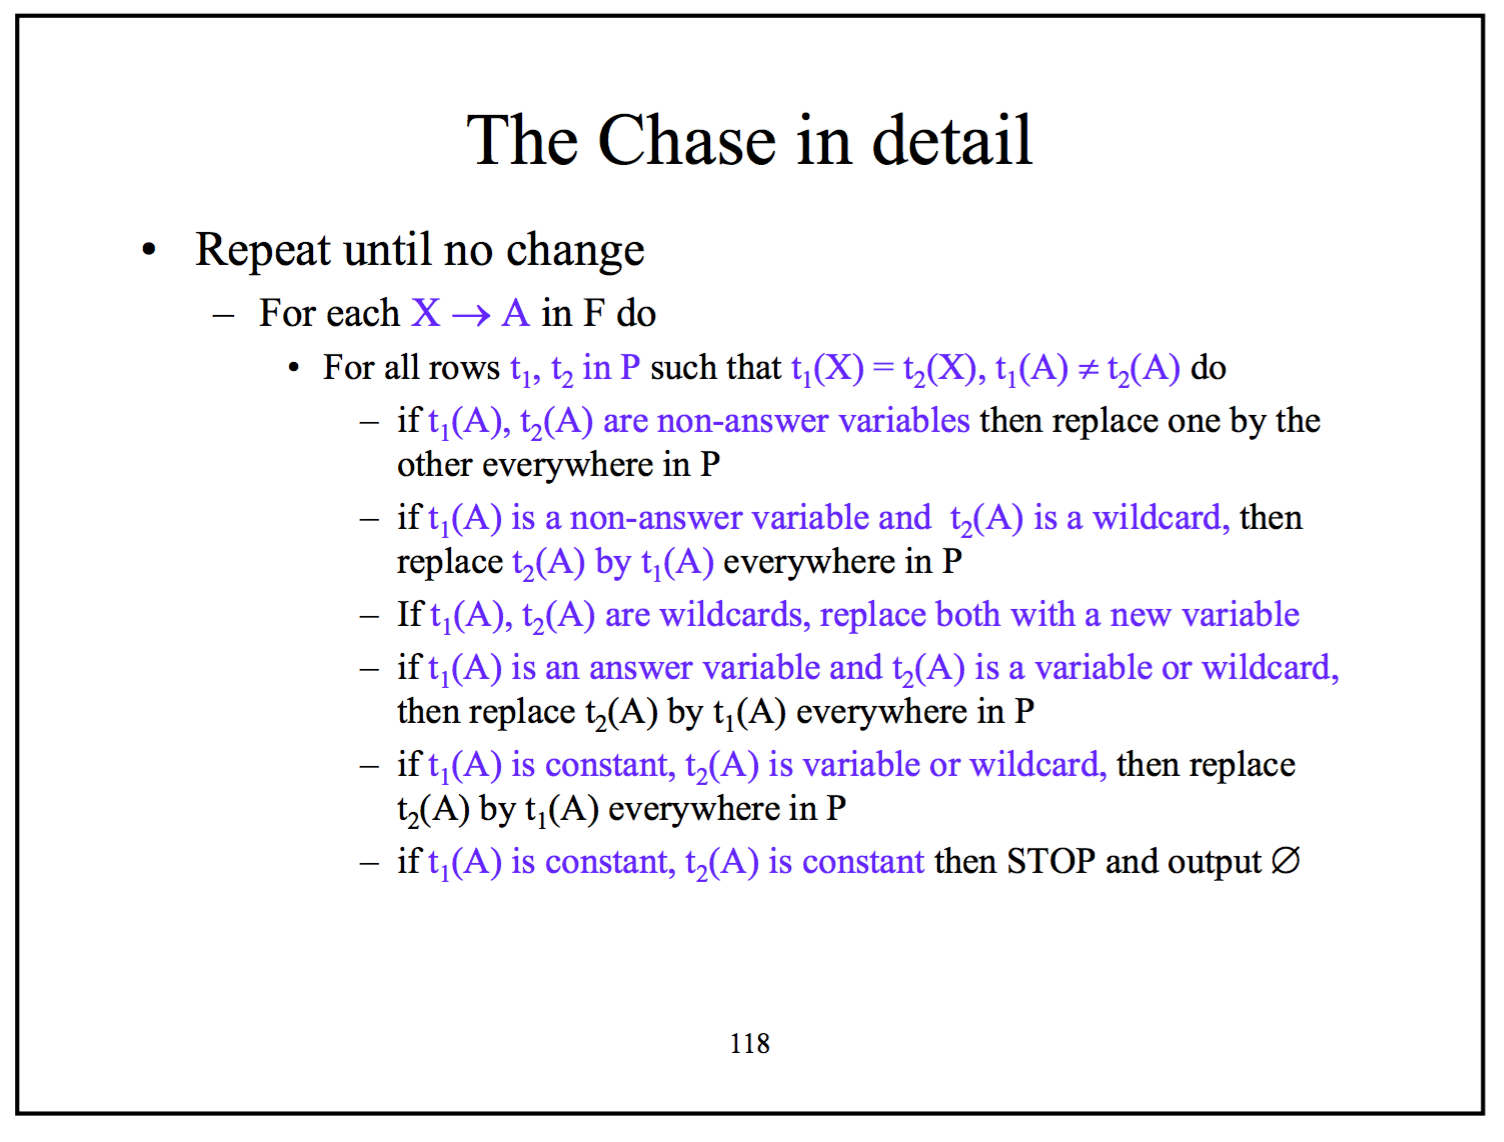
\includegraphics[scale=.80]{chase}}
\end{figure}
\end{frame}

\begin{frame}
  \frametitle{Example 2}
  Dependencies: $F = \{AC \rightarrow B, B \rightarrow C, C \rightarrow A \}$\\
  \begin{tabular}{ c | c c c}
  R & A & B & C \\
  \hline
  & \textcolor{red}{a}  & -  & c1 \\
  & -  & \textcolor{red}{b}  & c1 \\
  & a1 & \textcolor{red}{b} & - \\
  & a1 & - & \textcolor{red}{c} \\
  \end{tabular}
  \begin{tabular}{ c | c c c}
  answer & A & B & C \\
  \hline
   & \textcolor{red}{a}& \textcolor{red}{b}& \textcolor{red}{c}\\
  \end{tabular}
\end{frame}

\begin{frame}
  \frametitle{Example 2}
  Dependencies: $F = \{AC \rightarrow B, B \rightarrow C, C \rightarrow A \}$\\
  Use $B \rightarrow C$\\
  \begin{tabular}{ c | c c c}
  R & A & B & C \\
  \hline
  & \textcolor{red}{a}  & -  & c1 \\
  & -  & \textcolor{red}{b}  & c1 \\
  & a1 & \textcolor{red}{b} & - \\
  & a1 & - & \textcolor{red}{c} \\
  \end{tabular}
  \begin{tabular}{ c | c c c}
  answer & A & B & C \\
  \hline
   & \textcolor{red}{a}& \textcolor{red}{b}& \textcolor{red}{c}\\
  \end{tabular}
\end{frame}

\begin{frame}
  \frametitle{Example 2}
  Dependencies: $F = \{AC \rightarrow B, B \rightarrow C, C \rightarrow A \}$\\
  Use $C \rightarrow A$\\
  \begin{tabular}{ c | c c c}
  R & A & B & C \\
  \hline
  & \textcolor{red}{a}  & -  & c1 \\
  & -  & \textcolor{red}{b}  & c1 \\
  & a1 & \textcolor{red}{b} & c1 \\
  & a1 & - & \textcolor{red}{c} \\
  \end{tabular}
  \begin{tabular}{ c | c c c}
  answer & A & B & C \\
  \hline
   & \textcolor{red}{a}& \textcolor{red}{b}& \textcolor{red}{c}\\
  \end{tabular}
\end{frame}

\begin{frame}
  \frametitle{Example 2}
  Dependencies: $F = \{AC \rightarrow B, B \rightarrow C, C \rightarrow A \}$\\
  Eliminate rows\\
  \begin{tabular}{ c | c c c}
  R & A & B & C \\
  \hline
  & \textcolor{red}{a}  & -  & c1 \\
  & \textcolor{red}{a}  & \textcolor{red}{b}  & c1 \\
  & \textcolor{red}{a}  & \textcolor{red}{b} & c1 \\
  & \textcolor{red}{a}  & - & \textcolor{red}{c} \\
  \end{tabular}
  \begin{tabular}{ c | c c c}
  answer & A & B & C \\
  \hline
   & \textcolor{red}{a}& \textcolor{red}{b}& \textcolor{red}{c}\\
  \end{tabular}
\end{frame}

\begin{frame}
  \frametitle{Example 2}
  Dependencies: $F = \{AC \rightarrow B, B \rightarrow C, C \rightarrow A \}$\\
  Can we use any Dependencies?\\
  \begin{tabular}{ c | c c c}
  R & A & B & C \\
  \hline
  & \textcolor{red}{a}  & \textcolor{red}{b} & c1 \\
  & \textcolor{red}{a}  & - & \textcolor{red}{c} \\
  \end{tabular}
  \begin{tabular}{ c | c c c}
  answer & A & B & C \\
  \hline
   & \textcolor{red}{a}& \textcolor{red}{b}& \textcolor{red}{c}\\
  \end{tabular}
\end{frame}
\begin{frame}[fragile]
  \frametitle{Example 2}
  Dependencies: $F = \{AC \rightarrow B, B \rightarrow C, C \rightarrow A \}$\\
  \begin{tabular}{ c | c c c}
  R & A & B & C \\
  \hline
  & \textcolor{red}{a}  & \textcolor{red}{b} & - \\
  & \textcolor{red}{a}  & - & \textcolor{red}{c} \\
  \end{tabular}
  \begin{tabular}{ c | c c c}
  answer & A & B & C \\
  \hline
   & \textcolor{red}{a}& \textcolor{red}{b}& \textcolor{red}{c}\\
  \end{tabular}
  \hfill \\
\begin{verbatim} 
  SELECT r1.A, r1.B, r2.C
  FROM R r1, R r2
  WHERE r1.a = r2.a;
\end{verbatim}  
\end{frame}


\section{Reference}
\begin{frame}[fragile]
\frametitle{Reference}
\begin{enumerate}
\item ``\textit{Database Systems Concepts}'' by Silberschatz, Korth and Sudarshan, 6th edition, McGraw-Hill.
\end{enumerate}
\end{frame}


\begin{frame}[fragile]
  \frametitle{Example 3}
  Given the following pattern, minimize the pattern. 
\begin{verbatim}
SELECT t1.A, s1.E FROM R t1, R t2, R t3, R t4
S s1, S s2 WHERE 
  t1.B=t2.B AND t2.C=t3.C AND
  t3.A=t4.A AND t4.B=s2.B AND
  s2.D=s1.D;
\end{verbatim}
  
  \begin{tabular}{ c | c c c}
  R & A & B & C \\
  \hline
  t1 & $\alpha$  & b1  & - \\
  t2 & -  & b1  & c \\
  t3 & a & - & c \\
  t4 & a  & b & - \\
  \end{tabular}
   \begin{tabular}{ c | c c c}
  S & B & D & E \\
  \hline
  s1 & -  & d  & $\varepsilon$ \\
  s2 & b  & d  & - \\
  \end{tabular}
  \begin{tabular}{ c | c c c}
  answer & A & E \\
  \hline
   & $\alpha$& $\varepsilon$\\
  \end{tabular}
\end{frame}

\begin{frame}
  \frametitle{Example 3}

  \begin{tabular}{ c | c c c}
  R & A & B & C \\
  \hline
  t1 & $\alpha$  & b1  & - \\
  t2 & -  & b1  & c \\
  t3 & a & - & c \\
  t4 & a  & b & - \\
  \end{tabular}
   \begin{tabular}{ c | c c c}
  S & B & D & E \\
  \hline
  s1 & \textbf{b'}  & d  & $\varepsilon$ \\
  s2 & b  & d  & - \\
  \end{tabular}
  \begin{tabular}{ c | c c c}
  answer & A & E \\
  \hline
   & $\alpha$& $\varepsilon$\\
  \end{tabular}
\end{frame}

\begin{frame}
  \frametitle{Example 3}

  \begin{tabular}{ c | c c c}
  R & A & B & C \\
  \hline
  t1 & $\alpha$  & b1  & - \\
  t2 & -  & b1  & c \\
  t3 & a & - & c \\
  t4 & a  & \textbf{b'} & - \\
  \end{tabular}
   \begin{tabular}{ c | c c c}
  S & B & D & E \\
  \hline
  s1 & b'  & d  & $\varepsilon$ \\
  \end{tabular}
  \begin{tabular}{ c | c c c}
  answer & A & E \\
  \hline
   & $\alpha$& $\varepsilon$\\
  \end{tabular}
\end{frame}


\begin{frame}
  \frametitle{Example 3}

  \begin{tabular}{ c | c c c}
  R & A & B & C \\
  \hline
  t1 & $\alpha$  & b1  & - \\
  t2 & -  & b1  & c \\
  t3 & a & \textbf{b''} & c \\
  t4 & a  & b' & - \\
  \end{tabular}
   \begin{tabular}{ c | c c c}
  S & B & D & E \\
  \hline
  s1 & b'  & d  & $\varepsilon$ \\
  \end{tabular}
  \begin{tabular}{ c | c c c}
  answer & A & E \\
  \hline
   & $\alpha$& $\varepsilon$\\
  \end{tabular}
\end{frame}


\begin{frame}
  \frametitle{Example 3}

  \begin{tabular}{ c | c c c}
  R & A & B & C \\
  \hline
  t1 & $\alpha$  & b1  & - \\
  t2 & -  & b1  & c \\
  t3 & a & b'' & c \\
  \end{tabular}
   \begin{tabular}{ c | c c c}
  S & B & D & E \\
  \hline
  s1 & \textbf{b''}  & d  & $\varepsilon$ \\
  \end{tabular}
  \begin{tabular}{ c | c c c}
  answer & A & E \\
  \hline
   & $\alpha$& $\varepsilon$\\
  \end{tabular}
\end{frame}

\begin{frame}
  \frametitle{Example 3}

  \begin{tabular}{ c | c c c}
  R & A & B & C \\
  \hline
  t1 & $\alpha$  & b1  & - \\
  t2 & -  & b1  & c \\
  \end{tabular}
   \begin{tabular}{ c | c c c}
  S & B & D & E \\
  \hline
  s1 & \textbf{b1}  & d  & $\varepsilon$ \\
  \end{tabular}
  \begin{tabular}{ c | c c c}
  answer & A & E \\
  \hline
   & $\alpha$& $\varepsilon$\\
  \end{tabular}
\end{frame}
\begin{frame}
  \frametitle{Example 3}

  \begin{tabular}{ c | c c c}
  R & A & B & C \\
  \hline
  t1 & $\alpha$  & b1  & - \\
  \end{tabular}
   \begin{tabular}{ c | c c c}
  S & B & D & E \\
  \hline
  s1 & b1  & \textbf{-}  & $\varepsilon$ \\
  \end{tabular}
  \begin{tabular}{ c | c c c}
  answer & A & E \\
  \hline
   & $\alpha$& $\varepsilon$\\
  \end{tabular}
\end{frame}
\end{document}
